\documentclass[12pt,a4paper]{article}
\usepackage{hyperref}
\usepackage{amsmath}
\usepackage{amsthm}
\usepackage{amssymb}
\usepackage{gensymb}
\usepackage[margin=1.0in]{geometry}
\usepackage[T1]{fontenc}
\usepackage[utf8]{inputenc}
\usepackage{graphicx}
\usepackage{url}
\usepackage{placeins}
\usepackage{xcolor}
\usepackage{subcaption}
\usepackage{pgffor}
\captionsetup{compatibility=false}
\usepackage{setspace}
\usepackage{listings}
\usepackage{fontspec}
\setmainfont{URW Palladio L}
\linespread{1.05}         % Palladio needs more leading (space between lines)

\usepackage[style=numeric,backend=bibtex]{biblatex}
\addbibresource{temp.bib}
\graphicspath{ {./images/} }


\includeonly{
    contents/1-introduction,
    contents/2-theoretical-background,
    contents/3-symmetry-implementation,
    contents/4-experiments
}

\listfiles

\begin{document}
%--------------------------------------
% Strona tytułowa
%--------------------------------------
%\frontmatter
\begin{titlepage}
   \begin{center}
       \vspace*{0.5cm}
POZNAŃ UNIVERSITY OF TECHNOLOGY \\
FACULTY OF COMPUTING AND TELECOMMUNICATIONS \\
       INSTITUE OF COMPUTING \\

       \vspace*{2cm}
       {\Large MASTER THESIS} \\

       \vspace*{1cm}
       \textbf{\Huge Equivariant neural networks for image recognition}  \normalfont \\

       \vspace{5cm}
       \begin{doublespace}
       Author: \\
       {\Large Kamil Burdziński} \\
       \end{doublespace}
       \vspace{4cm}
       \begin{doublespace}
       Tutor:\\
       {\Large dr hab. inż. Wojciech Kotłowski}
       \end{doublespace}
   \end{center}
\end{titlepage}

% Front matter starts here
\cleardoublepage%

%--------------------------------------
% Dedication page
%--------------------------------------

\thispagestyle{empty}
\vspace*{\fill}%
\vspace{17cm}
\begin{flushright}
\textit{Dedication page}
\end{flushright}
\vfill\cleardoublepage%

% -- table of contents --
\tableofcontents
\thispagestyle{empty}

\cleardoublepage % Zaczynamy od nieparzystej strony
\pagenumbering{arabic}

% --- Main Document --- --- --- --- --- --- ---
%
\section{Introduction}
\subsection{Background}
The last couple \WK{of} years saw a rapidly surging interest in neural networks
invariant to certain groups of transformations. This property
is very much sought after because under mild assumptions it
guarantees the output of the network won't change when transformed according to
chosen
transformations. Related desirable quality of neural networks is equivariance
which on the other hand causes output to change in the same way the input
changes. Growing body of work presents wide variety of
techniques applied to ensure these properties.
\\ However so far almost all of published papers focused exclusively on
geometric symmetries of images, e.g. rotations, scaling or reflection. Transforms
related to lightning of the image, like contrast or brightness have been largely
ignored.
\subsection{Objectives}
In this work we address the following problems:
\begin{enumerate}
    \item Is constructing neural networks either equivariant or invariant to
        lightning symmetries feasible? If so then how do they compare to networks
        lacking these properties?
    \item What's the degree of equivariance of such models? Is the equivariance
        exact or does inevitable discretization impose significant error?
        Does it differ significantly from equivariance to geometric
        transformations? \WK{last sentence unclear}
\end{enumerate}
In order to answer these questions, we carry out the following tasks:
\begin{enumerate}
    \item Possibly extending notions of contrast, brightness, gamma correction 
        and color balance from
        images to tensors of arbitrary dimensionality.
    \item Constructing neural network layers invariant to various lightning
        symmetries.
    \item Adapting existing architectures to ensure equivariance to some or
        possibly all of mentioned lightning transformations.
    \item Comparing constructed models with control group on image
        classification tasks.
    \item Estimating numerically degree of invariance and equivariance of constructed models.
\end{enumerate}

\section{Theoretical background}

\subsection{Group theory}
    \textbf{Group} $G$ is a set together with binary operation $\left(G, \bullet \right)$ satisfying
    following axioms:
    \begin{enumerate}
        \item Closure: for any $g, h \in G$, $g \bullet h \in G$
        \item Associativity:  $g\bullet \left(h \bullet j \right) =
                    \left(g \bullet h \right) \bullet j$ for any $g,h,j \in G$
        \item Identity: there exists a neutral element $e$ such that
                $e \bullet g = g \bullet e = g$ for any $g \in G$
        \item Inverse element: for every $g \in G$ exists element $h \in G$ such that
                $g \bullet h = h\bullet g = e$. The element inverse to $g$ is usually
                written as $g^{-1}$
    \end{enumerate}
    \par Group $G$ might also posses additional structure. A \textbf{topological group}
        is a group together with a topology on G, such that $G$'s binary operation:\\
        \hspace*{0.5cm} $\bullet: G \times G \to G, \left(g,h \right) \mapsto g\bullet h$ \\
        and inversion map: \\
        \hspace*{0.5cm} ${}^{-1}: G \to G, g \mapsto g^{-1}$ \\
        are continuous. Additionally if the underlying topological structure
        is some smooth n-manifold and both maps are smooth, the group is called
        \textbf{Lie group}. Familiar examples of Lie groups include translation group
        $\left( \mathbb{R}^n, + \right)$ - set of real vectors with addition or
        $\left(GL(n,\mathbb{R}), \cdot \right)$ - set of real $n \times n$ matrices of nonzero determinant
        with multiplication.\\\par
        Just as we can form functions between sets assigning elements of one set to
        the elements of other, it's possible to construct functions between groups.
        Typically we are interested in functions preserving to some extent the group structure,
        that is of the form.
        \begin{equation}
            f:G \to H, \hspace{1cm} f(x\bullet y) = f(x) \ast f(y)
        \end{equation}
        where $\bullet$ is the binary operation in group $G$ and $\ast$ is the binary operation
        in group $H$. Such functions are called \textbf{group homomorphisms}.
        Bijective homomorphism is called \textbf{isomorphism}.\\

        In this work we are mainly interested in groups in context of their actions
        on 3D tensors. Given a group $G$ and set $X$ we define a
        \textbf{group action} of $G$ on $X$ as a function
        \begin{equation}
            \theta: G \times X \to X
        \end{equation}
        (with $\theta(g,x)$ often written as $g\cdot x$) satisfying following axioms:
        \begin{enumerate}
            \item Identity: $e \cdot x = x$ for every $x \in X$, where $e$ is the neutral element
                    of $G$
            \item Compatibility: $g \cdot \left(h \cdot x\right) =
                \left(g \bullet h \right) \cdot x$ for all $g$ and $h$ in $G$ and $x$ in $X$
        \end{enumerate}
        The simplest possible group action is the trivial group action, that is
        $g\cdot x = x$ for any $g$ and $x$. Familiar nontrivial examples include isometries
        of $\mathbb{R}^n$, e.g.
        translations - action of $\left(\mathbb{R}^n,+\right)$ given by $v \cdot x = v+x$ or
        rotations - action of $SO(n,\mathbb{R})$ given by $r \cdot x = Rx$ where
        $R$ is matrix representation of rotation and
        multiplication on the right is matrix-vector multiplication.\\
        Now suppose we are given some function $f:G\to \mathbb{R}^n$.
        We can define natural action of $G$ on set of such functions by:
        \begin{equation}
            (g\cdot f)(x) = f(g^{-1}\bullet x)
            \label{eq:action_on_function}
        \end{equation}
        It's a group action because:
        \begin{align*}
            & (e\cdot f)(x) = f(e\bullet x) = f(x) \\
            & \mbox{and} \\
            & ((g\bullet h) \cdot f)(x) = f((g\bullet h)^{-1} \bullet x) =
            f(h^{-1}\bullet g^{-1} \bullet x) = (h\cdot f)(g^{-1} \bullet x) =
            (g\cdot(h \cdot f))(x)
        \end{align*}








\subsection{Equivariant and invariant neural networks}
    \subsubsection{Equivariant and invariant maps}
    \label{sec:theoretical_equiinv}
    \hspace{0.5cm}
     Key properties of neural networks in regard to group actions are equivariance and invariance.
        These can be abstractly defined as follows: \par
        Let group $G$ act on sets $X$ and $Y$. We call function $f: X \rightarrow Y$ equivariant
        with respect to action of $G$ if for all $g \in G$ and $x \in X$
        \begin{equation}
            f(g \cdot x) = g \cdot f(x)
        \end{equation}
        In turn, we call $f$ invariant with respect to action of $G$ if
        \begin{equation}
            f(g \cdot x) = f(x)
        \end{equation}
        In fact invariance is a special case of equivariance where action of $G$ on $Y$ is trivial.
        It's however conceptually cleaner to make distinction between both properties.
        Intuitively equivariance tells us that when input changes, the output changes accordingly
        and invariance -- that action of G has no effect on output.\par
            If we want to construct a neural network $\mathcal{N}$ equivariant to some
        specified group action, we need to make sure each of it's layers is equivariant.
        If we treat $\mathcal{N}$ as a series of functions $f_0,f_1,...,f_n$, then
        \begin{align*}
            \mathcal{N}(g \cdot x) &=
            f_n \circ f_{n-1} \circ \cdots \circ f_1 \circ f_0(g\cdot x)  \\
            &= f_n \circ f_{n-1} \circ \cdots \circ f_1 \circ \left( g \cdot f_0(x) \right) \\
            &= \cdots \\
            &= g \cdot f_n \circ f_{n-1} \circ \cdots \circ f_1 \circ f_0(x) \\
            &= g \cdot \mathcal{N}(x)
        \end{align*}
        where $g\cdot x$ is the action of $g$ on $x$. Often we don't want the network
        to be fully equivariant; the desired extent of equivariance depends on the task.
        For problems of image-to-image type like segmentation full equivariance is desirable.
        However for problems where the input data gets more and more ``squished'' in consecutive layers,
        we need to break equivariance at some point. Like for example in classification,
        where final layers are often fully connected and not equivariant. \par
        The easiest way to assert the network is invariant to some transformation
        is making it's very first layer $f_0$ invariant, then:
        \begin{align*}
            \mathcal{N}(g\cdot x)
            &= f_n \circ f_{n-1} \circ \cdots \circ f_1 \circ f_0(g\cdot x)  \\
            &= f_n \circ f_{n-1} \circ \cdots \circ f_1 \circ f_0(x) \\
            &= \mathcal{N}(x)
        \end{align*}
        Equivalently one can make the couple first layers equivariant and a single layer
        following them invariant. For example if $f_0$ is equivariant and $f_1$ invariant we get:
        \begin{align*}
            \mathcal{N}(g\cdot x)
            &= f_n \circ f_{n-1} \circ \cdots \circ f_1 \circ f_0(g\cdot x)  \\
            &= f_n \circ f_{n-1} \circ \cdots \circ f_1 \circ \left( g \cdot f_0(x) \right) \\
            &= f_n \circ f_{n-1} \circ \cdots \circ f_1 \circ f_0(x) \\
            &= \mathcal{N}(x)
        \end{align*}
        and the network is again invariant. Modern literature is often not so
        clear regarding terminology and networks of the above type are sometimes
        also called equivariant.

    \subsubsection{GCNN}
    The primary example of equivariant neural networks are convolutional neural
    networks which are (roughly) equivariant to translations. The $4$ basic
    components of CNN are convolutional layers, pooling layers, normalization
    layers and activation functions.  These common building are approximately
    equivariant to translations:
    \begin{itemize}
        \item Convolutional layer is
            equivariant outside of image's borders. The border effects can to
            some extent be fixed by padding image with values present in the
            border or their averages.
        \item Max pooling layer is locally invariant -- that is small translations don't
            affect the layer's output, but translations which are multiplicities
            of window's size cause equivariant behaviour.
            In average pooling local behaviour is more
            complicated, but they are also equivariant to window-sized
            translations.
        \item Usual normalization schemes like batch or instance
            normalization depend on global statistics
            like mean and standard deviation which change slightly during
            translation so their are not exactly equivariant. However given
            proper padding method these changes can be very small if
            translation is not too big.
        \item Activation functions are applied pointwise so, they are
            perfectly equivariant outside borders.
    \end{itemize}
    Of course the most crucial parts of CNN are convolution layers. At each
    layer CNN takes as input 3-dimensional tensor which can be thought of as a
    stack of functions $f:\mathbb{Z}^2\to\mathbb{R}^C$ where $C$ is number of channels.
    Convolutional layer correlates it with a set of filters $\psi^i$
    and each filter can also be thought of as a stack of functions
    $\psi^i:\mathbb{Z}^2\to\mathbb{R}^C$:
    \begin{equation}
        \label{eq:cnn}
        (f\star\psi^i)(x) = \sum_{y\in\mathbb{Z}^2}\sum_{c=1}^C
        f_c(y)\psi_{c}^{i}(y-x)
    \end{equation}

    By generalizing convolutions and architecture of CNNs we would like to
    construct models
    equivariant or invariant to some specified set of image transformations.
    One of the earliest works on this problem appeared in \cite{cohen2016}. There
    the so called \textit{Group Equivariant Convolutional Neural Networks}
    (G-CNNs) equivariant to possibly any discrete set of transformations were
    proposed. Their main idea is generalizing the convolution layer by
    lifting tensors the network operates on to higher dimensions.
    Just like traditionally the last two
    dimensions encode height and width, these new dimensions can
    encode information about the chosen group of transformations. These higher
    dimensional tensors are then thought of as stacks of functions
    $F:G\to\mathbb{R}^C$, where $G$ is the group of transformations.
    Pictures \ref{fig:p4_rot} and \ref{fig:p4m_rot} show
    feature maps for $p4$ -- group of translations and rotations and for
    $p4m$ -- group of
    translations, rotations and reflections.
    Convolutional filters of respective GCNNs are shaped in the same way
    but their heights and widths are smaller (typically $3\times3$ or $5\times5$
    just like in normal CNNs).
    \begin{figure}[h]
        \centering
        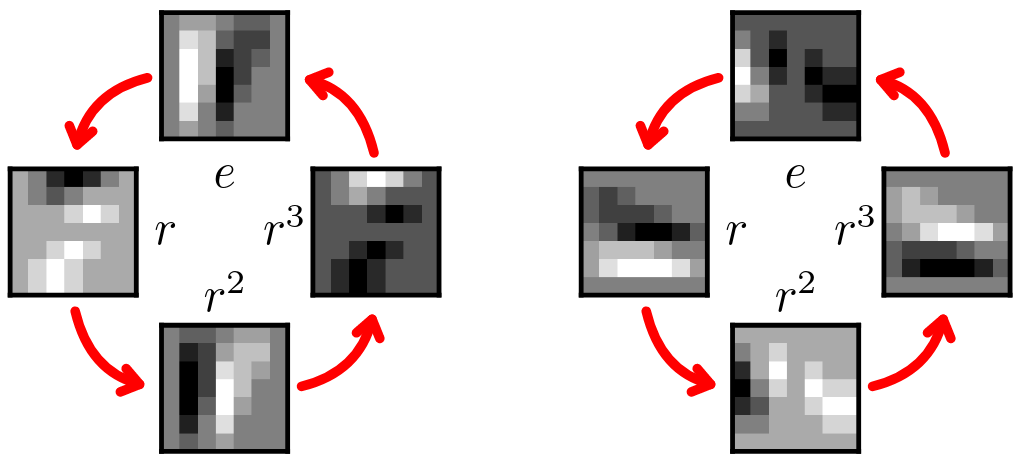
\includegraphics[width=0.7\textwidth]{p4_rot}
        \caption{On the left: schematic representation of feature map $F$ flowing through
            p4-equivariant GCNN. Computationally $F$ can be thought of as tensor of shape
            $4\times H \times W$, where each of $4$ submaps represents one of
            rotations by $0\degree$, $90\degree$, $180\degree$ or $270\degree$.
            On the right, the same feature map rotated by
            $90 \degree$ counterclockwise -- $r\cdot F$ in the sense of equation
            \ref{eq:action_on_function}. Note that every submap follows the
            red arrow as well as gets rotated. This stems from the structure of
            $p4$ group.}
        \label{fig:p4_rot}
    \end{figure}
    \begin{figure}[h]
        \centering
        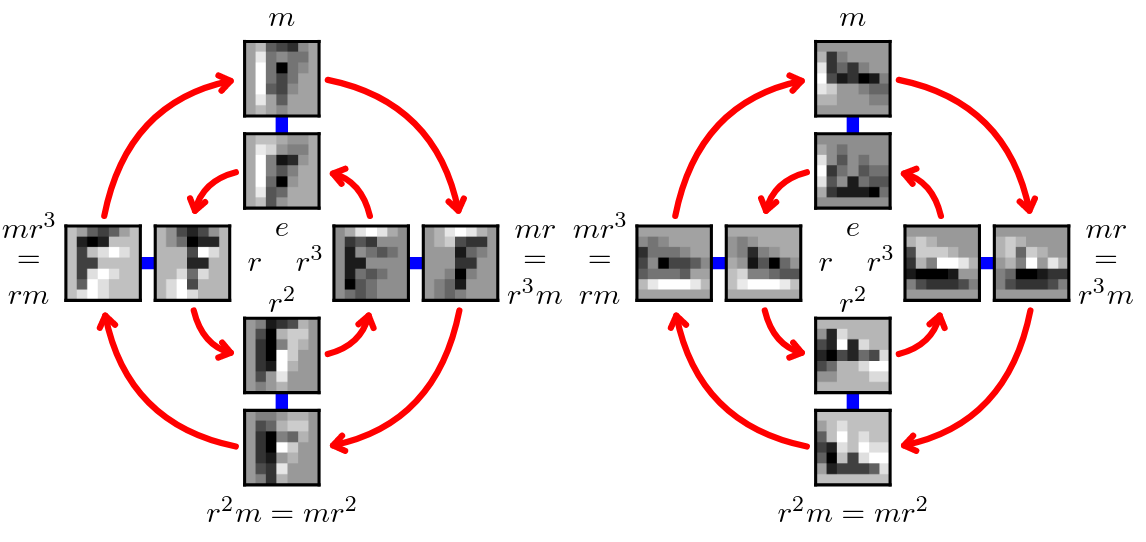
\includegraphics[width=0.7\textwidth]{p4m_rot}
        \caption{Feature map of p4m-equivariant GCNN and it's rotation by $r$.}
        \label{fig:p4m_rot}
    \end{figure}

    \textbf{Lift} operation is a particular kind of convolution
    that transforms usual function stack $f$ on $\mathbb{Z}^2$ into
    function stack $F$ on group $G$. Computationally it takes as input
    usual 3d tensor (channel, height, width) and produces
    N-dimensional tensor with $N>3$:
    \begin{equation}
        \label{eq:gcnn-lift}
        \mathit{Lift}(f)(g) = F(g) = (f\star\psi^i)(g) = \sum_{y\in \mathbb{Z}^2}\sum_{c=1}^C
        f_c(y)\psi_{c}^{i}(g^{-1}y)
    \end{equation}
    Once the input tensor is lifted, in consecutive convolutional layers it
    undergoes \textbf{group convolutions}:
    \begin{equation}
        \label{eq:gcnn}
        F(g) = (f\star\psi^i)(g) = \sum_{y\in G}\sum_{c=1}^C
        f_c(y)\psi_{c}^{i}(g^{-1}y)
    \end{equation}
    Note that while in equation \ref{eq:cnn} computation is done by sliding
    $y$ on $\mathbb{Z}^2$, in equation \ref{eq:gcnn} it's replaced by more
    general iteration on all group elements. If we replace $G$ by $\mathbb{Z}^2$
    and set $g=x$ we obtain equation \ref{eq:cnn} back since in $\mathbb{Z}^2$,
    $x^{-1}$ is just $-x$. We can prove operator defined by equation
    \ref{eq:gcnn} is equivariant to action of any element $h$ of $G$:
    \begin{align*}
        ((h\cdot f)\star\psi)(g) & =
        \sum_{y\in G}\sum_{c=1}^C f_c(h^{-1}y)\psi_{c}(g^{-1}y)\\
        & = \sum_{hy\in G}\sum_{c=1}^C f_c(y)\psi_{c}(g^{-1}hy)\\
        & = \sum_{hy\in G}\sum_{c=1}^C f_c(y)\psi_{c}((h^{-1}g)^{-1}y)\\
        & = (f\star\psi)(h^{-1}g) &  \\
        & = (h\cdot(f\star\psi))(g)
    \end{align*}
    The proof goes similarly for equation \ref{eq:gcnn-lift}.

    The ideas contained in \cite{cohen2016} were further generalized to new
    possible groups of transformations, domains and neural network
    architectures. \cite{cohen_spherical_cnns, kondor_trivedi,
    esteves_so3} describe convolutional layers equivariant to
    the group of 3-dimensional rotations $\mathit{SO}(3)$.
    They make heavy use of spherical harmonics for parametrization and
    speedup of computation. Equivariance to $\mathit{SO}(3)$ is beneficial
    in any tasks regarding real world environments like depth estimation or 3d
    objects classification\cite{esteves_so3}. It helps also by
    prediction of properties of
    molecules described in terms of 3d-coordinates \cite{lieconv}.
    In less obvious way
    $\mathit{SO}(3)$-equivariant GCNNs are used to process data whose natural
    domain is spherical, e.g. Earth weather data or images from drone camera
    \cite{cohen_spherical_cnns}.

    

    \cite{bekkers2019, lieconv} propose general frameworks for
    GCNNs equivariant to any Lie group whereas \cite{cohen2016} only really
    touched on finite groups. That's important since many natural
    transformations of data are continuous and often have structure of Lie group
    like group of all rotations of plane ($SO(2)$), rotations of sphere
    ($SO(3)$) or scaling of images $(R_+, \times)$.


\subsection{Image symmetries}
    \label{sec:transformations}
    In this section we define and generalize symmetries of images that we wish
    neural networks to respect. First we describe
    properties related to lightning in image - contrast,
    brightness, color balance and gamma correction. Then geometric operators -
    rotations, scaling and shear - are presented.
    Throughout this section and for the rest of the work,
    ``image'' is understood to be an array of
    floating point numbers in range $\left[0;1\right]$ of shape $\left(3, H,
    W\right)$.
    \subsection{Lightning operators}
    \subsubsection{Contrast}
    \newcommand\mcc{\mathcal{C}}
        The usual formula for changing image's contrast by factor of $a$ is
        \begin{equation}
            \label{eq:contrast_old}
        C_a(X) = \mathit{CLIP}\left(a\cdot X + (1-a) \cdot E\left[ \frac{w_1X_r
        + w_2X_g + w_3X_b}{w_1+w_2+w_3}\right]   \right)
        \end{equation}
        where
        $\mathit{CLIP}$ is function clipping values to $\left[0;1\right]$ range,
        $X_r, X_g$ and $X_b$ are red, green and blue channels of the image and
        the expectation on the right is mean value of grayscale version of
        image.  Grayscale is understood to be a weighted average of image's
        channels.  Changing the contrast by factor of $1$ has no effect, using
        the factor of $2$ is supposed to double the contrast, factor of $0.5$
        halves the contrast, etc.  This definition however is not suitable for
        usage in the context of neural networks.  First of all it assumes the
        tensor has 3 channels, while we would like to have a definition
        independent of number of channels. The concept of green channel or red
        channel also doesn't exist for tensors with more channels. Therefore we
        choose to generalize the definition by replacing weighted average with
        usual average. The second problem is clipping values. Working only with
        values in range $\left[0;1\right]$ at all times would make training a
        neural network a lot harder and perhaps significantly diminish it's
        performance. To avoid these effects we entirely give up on clipping
        values.  The final formula for changing contrast is following:
        \begin{equation}
            \label{eq:contrast}
            \mathcal{C}_a(x) = ax + (1-a) \mu_x
        \end{equation}
        where $\mu_x$ is the average value of whole tensor. It's however worth
        noting, that removing the clipping changes the general behavior of the
        transformation.  While it remains more or less unchanged for values of
        $a$ close to $1$, differences grow as me move further away from identity
        transformation.
        % TODO: plot of difference between original definition and the adopted definition

        This operator possesses a number of interesting properties:
        \begin{itemize}
            \item $\mathcal{C}_a$ is linear operator on vector space of images of fixed size:
                \begin{align*}
                    & \mathcal{C}_a(x+y) =
                    a(x+y) + (1-a)\mu_{x+y} =
                    ax + ay +(1-a)\mu_x +(1-a)\mu_y =
                \mathcal{C}_a(x) + \mathcal{C}_a(y) \\
                    & \mathcal{C}_a(\lambda x) = a\lambda x + (1-a)\mu_{\lambda x} =
                    \lambda ax + (1-a)\lambda\mu_x = \lambda(ax + (1-a)\mu_x) =
                    \lambda \mathcal{C}_a(x)
                \end{align*}

            \item Under map composition, set
                $\mathcal{C} = \left\{\mathcal{C}_a | a\in \mathbb{R}_+\right\}$
                forms a Lie group isomorphic to $\left(\mathcal{R}_+,\cdot \right)$ -- set of
                positive real numbers with multiplication:
                \begin{enumerate}
                    \item Closure:\\
                        $\mathcal{C}_a\circ \mathcal{C}_b(x) =
                \mathcal{C}_a(bx + (1-b)\mu_x) =
                abx + a(1-b)\mu_x + (1-a)\mu_{bx+(1-b)\mu_x} =
                abx + a(1-b)\mu_x + (1-a)b\mu_x + (1-a)(1-b)\mu_x=
                abx + (1-ab)\mu_x =
                \mathcal{C}_{ab}(x)$
                    \item Associativity:\\
                        $ \mcc_a \circ(\mcc_b \circ \mcc_c(x)) =
                            \mcc_a(\mcc_{bc}(x)) = \mcc_{abc}(x) =
                                \mcc_{ab}\circ\mcc_c(x) = (\mcc_a \circ \mcc_b) \circ\mcc_c(x)$
                    \item Identity:\\
                        $\mcc_1\circ\mcc_a(x) = \mcc_a\circ\mcc_1(x) =
                            \mcc_a(x)$
                    \item Inverse element:\\
                        $\mcc_a\circ\mcc_{a^{-1}}(x) = \mcc_{a^{-1}}\circ\mcc_a(x) = \mcc_1(x)$
                \end{enumerate}
                The homomorphism is simply $h: \mcc_a \mapsto a$
                $$ h(\mcc_a)h(\mcc_b) = ab = h(\mcc_{ab})$$
                It is bijective so it's isomorphism.

            \item Equation \ref{eq:contrast} defines a group action of $\mcc$ on space of images:
                $\mcc_1 \cdot x = 1x + (1-1)\mu_x = x$ and checking the compatibility axiom
                is the same as checking the closure axiom above.
            \item $\mcc_n$ increases standard deviation of image $n$ times:\\
                $\sigma(\mcc_n(x)) = \sigma(nx + (1-n)\mu_x) = \sigma(nx) = n\sigma(x)$
        \end{itemize}
        \par Visually the difference between operators using weighted and unweighted
        averages is small. Picture \ref{fig:contrast_pics} shows series of
        photographies from STL10 dataset with with varying contrast changes.

        \newcommand{\contrastpic}[3]{
            \begin{subfigure}{#3\textwidth}
                \includegraphics[width=\linewidth]{contrast_#1/#2}
            \end{subfigure}}
        \newcommand{\contrastpiccaption}[4]{
            \begin{subfigure}{#3\textwidth}
                \includegraphics[width=\linewidth]{{contrast_#1/#2}.jpg}
                \caption*{$a=#4$}
            \end{subfigure}}

        \begin{figure}[h]
            \centering
            \foreach \n in {0_1, 0_25, 0_5, 1, 2, 4,10}
                {\contrastpic{default}{0temp\n}{0.12}} \\
            \foreach \n in {0_1, 0_25, 0_5, 1, 2, 4,10}
                {\contrastpic{custom}{0temp\n}{0.12}} \\[1em]
            \foreach \n in {0_1, 0_25, 0_5, 1, 2, 4,10}
                {\contrastpic{default}{121temp\n}{0.12}} \\
            \foreach \n in {0_1, 0_25, 0_5, 1, 2, 4,10}
                {\contrastpic{custom}{121temp\n}{0.12}} \\[1em]
            \foreach \n in {0_1, 0_25, 0_5, 1, 2, 4,10}
                {\contrastpic{default}{105temp\n}{0.12}} \\
            \foreach \n in {0.1, 0.25, 0.5, 1, 2, 4,10}
                {\contrastpiccaption{custom}{105temp\n}{0.12}{\n}}

        \caption{Differences between weighted and unweighted contrast change
            operator. Top rows: $C_a$ operator (equation \ref{eq:contrast_old}.
            Bottom rows: $\mcc_a$ operator (equation \ref{eq:contrast} with
            clipping).}
        \label{fig:contrast_pics}
        \end{figure}


    \subsubsection{Brightness}
        Change in image brightness is defined similarly to change in contrast, except
        the subtraction of image's mean is skipped:
        \begin{equation}
            \label{eq:bright_old}
            B_a(X) = \mathit{CLIP}\left(aX\right)
        \end{equation}
        Again omitting the clipping, the brightness change operator is defined simply as
        \begin{equation}
            \label{eq:bright}
            \mathcal{B}_a(x) = ax
        \end{equation}
        All properties characterising the $\mcc$ operators listed above
        are also true for the set $\mathcal{B} = \{\mathcal{B}_a | a>0 \}$.
        It's worth noting, that in this case removing the clipping step doesn't change
        the definition so significantly. In fact both formulas agree as long as $a\leq 1$,
        that is as along as brightness is not increased.
        Picture \label{fig:brightness_pics} shows images with brightness varying
        according to equation \ref{eq:bright_old}.


        \newcommand{\brightnesspic}[2]{
            \begin{subfigure}{#2\textwidth}
                \includegraphics[width=\linewidth]{{brightness/#1}.jpg}
            \end{subfigure}}
        \newcommand{\brightnesspiccaption}[3]{
            \begin{subfigure}{#2\textwidth}
                \includegraphics[width=\linewidth]{{brightness/#1}.jpg}
                \caption*{$a=#3$}
            \end{subfigure}}

        \begin{figure}[h]
            \centering
            \foreach \n in {0.1, 0.25, 0.5, 1, 2, 4,10}
                {\brightnesspic{0temp\n}{0.12}} \\
            \foreach \n in {0.1, 0.25, 0.5, 1, 2, 4,10}
                {\brightnesspic{121temp\n}{0.12}} \\
            \foreach \n in {0.1, 0.25, 0.5, 1, 2, 4,10}
                {\brightnesspiccaption{105temp\n}{0.12}{\n}}

        \caption{Images from STL10 dataset with brightness changed with operator
            $B_a$.}
        \label{fig:brightness_pics}
        \end{figure}


        %TODO: insert the plot of mean value of transformed image depending on change
        % brightness




    \subsubsection{Color balance}
        Suppose we are given a 3-channel image represented as a list of channels
        $\left[ X_r, X_g, X_b\right]$. Then the operator changing the color balance
        to the balance corresponding to the temperature $T$ is defined as
        \begin{equation}
            \mathcal{W}_T \left(\left[ X_r, X_g, X_b \right]\right) =
            \left[T_r X_r, T_g X_g, T_b X_b \right]
        \end{equation}
        where $T_r, T_g, T_b$ are RGB components corresponding to temperature $T$.
        For example for $T=1000K$, $T_r, T_g$ and $T_b$ equal $1, 0.0401$ and $0$ respectively.
        $T$ ranges from $1000K$ to $40000K$ with steps of $100$
        though there is not much change after the $15000$ threshold.
        Figure \ref{fig:color_balance} shows part of possible temperature spectrum
        together with colors characterising temperatures in terms of uint8 RGB triplets.
        Picture \ref{fig:cb_pics} shows images with varying color balance.

        \begin{figure}[h]
            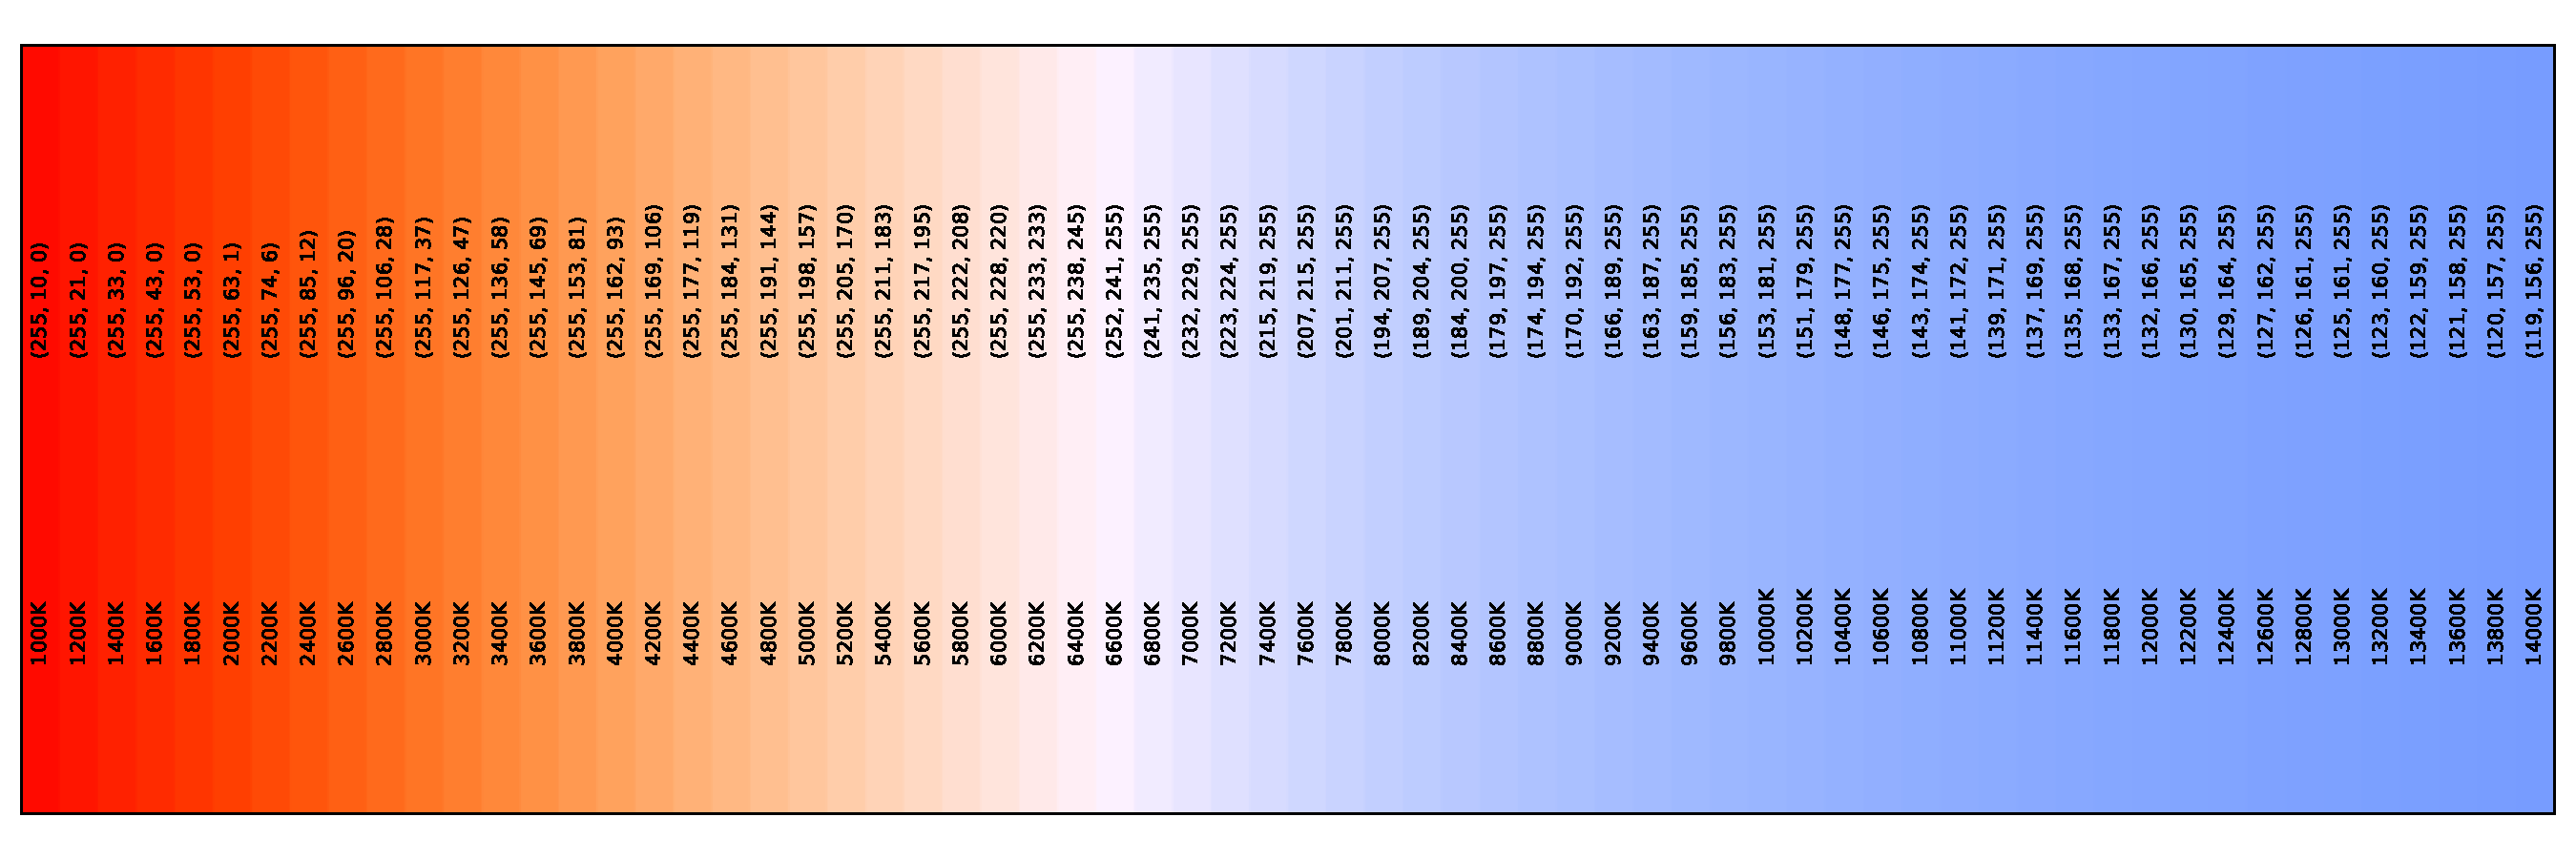
\includegraphics[width=\textwidth]{color_balance}
            \caption{}
            \label{fig:color_balance}
        \end{figure}

        \newcommand{\cbpic}[2]{
            \begin{subfigure}{#2\textwidth}
                \includegraphics[width=\linewidth]{{color_balance/#1}.jpg}
            \end{subfigure}}
        \newcommand{\cbpiccaption}[3]{
            \begin{subfigure}{#2\textwidth}
                \includegraphics[width=\linewidth]{{color_balance/#1}.jpg}
                \caption*{$T=#3K$}
            \end{subfigure}}

        \begin{figure}[h]
            \centering
            \foreach \n in {1000, 3000, 5000, 7000, 9000}
                {\cbpic{0temp\n}{0.18}} \\
            \foreach \n in {1000, 3000, 5000, 7000, 9000}
                {\cbpic{121temp\n}{0.18}} \\
            \foreach \n in {1000, 3000, 5000, 7000, 9000}
                {\cbpiccaption{105temp\n}{0.18}{\n}}

        \caption{Images from STL10 dataset with color balance changed with operator
            $\mathcal{W}_T$.}
        \label{fig:cb_pics}
        \end{figure}

        Unlike contrast or brightness, the color balance is inherently
        bound to colors of image, so it's very hard to come up with reasonable
        generalization to higher dimensions which would allow us to measure
        equivariance. We choose not to do that and instead only construct
        networks invariant to changes in color balance.

    \subsubsection{Gamma correction}
        Gamma correction of image X is defined as
        \begin{equation}
        G_a(X) = X^a
        \label{eq:simple_gamma}
        \end{equation}
        where $a \in \mathbb{R}_+$ and exponentiation is done entrywise.
        Figure \ref{fig:gamma_pics} shows examples of pictures with various gamma
        settings.

        \newcommand{\gammapic}[2]{
            \begin{subfigure}{#2\textwidth}
                \includegraphics[width=\linewidth]{{gammas/#1}.jpg}
            \end{subfigure}}
        \newcommand{\gammapiccaption}[3]{
            \begin{subfigure}{#2\textwidth}
                \includegraphics[width=\linewidth]{{gammas/#1}.jpg}
                \caption*{$a=#3$}
            \end{subfigure}}

        \begin{figure}[h]
            \centering
            \foreach \n in {0.33, 0.75, 1, 1.5, 3}
                {\gammapic{0temp\n}{0.18}} \\
            \foreach \n in {0.33, 0.75, 1, 1.5, 3}
                {\gammapic{121temp\n}{0.18}} \\
            \foreach \n in {0.33, 0.75, 1, 1.5, 3}
                {\gammapiccaption{105temp\n}{0.18}{\n}}

            \caption{Images from STL10 dataset with varying gamma settings.}
        \label{fig:gamma_pics}
        \end{figure}


        Unfortunately this definition is troublesome when applied to tensors
        with negative values as for example $a=\frac{1}{2}$ results in
        complex values. Also since every number has $n$ complex roots of degree
        $n$, a problem with selecting the proper root appears. In order to avoid
        these problems, we restrict computation to real numbers and generalize
        equation \ref{eq:simple_gamma} by:
        \newcommand\mcg{\mathcal{G}}
        \begin{equation}
            \mathcal{G}_a(X) = \mathit{sign}(X)\cdot|X|^a
            \label{eq:gamma}
        \end{equation}
        where $\mathit{sign}(X)$ is a tensor of the same shape as $X$ containing
        signs of it's entries and $|X|$ contains absolute values of entries.
        Exponentiation is again computed entrywise. This way we separate signs
        and magnitudes.
        \par Unlike the three previous operators, $\mathcal{G}_a$ is nonlinear --
        $(X+Y)^a \neq X^a + Y^a$ unless $a=1$. This family of transformations forms however a
        group under function composition $\mcg_a \circ \mcg_b = \mcg_{ab}$.
        It's isomorphic to $(\mathbb{R}_+, \cdot)$ with isomorphism $f$
        given by $f:\mcg_a \mapsto a$ and acts on the space of
        tensors of fixed shape:
        \begin{itemize}
            \item $\mathcal{G}_1(X) = X^1 = X$
            \item $\mcg_a\left(\mcg_b\left(X\right)\right) =
                \mcg_a\left(s\left(X\right)\cdot\left|X\right|^b\right) =
                s\left(s\left(X\right)\cdot\left|X\right|^b\right)
                \cdot\left|s\left(x\right)\cdot\left|X\right|^b\right|^a =
                s\left(s\left(X\right)\right)\cdot\left|\left|X\right|^b\right|^a
                = s\left(X\right)\cdot\left|X\right|^{ba} = \mcg_{ab}(X)$
        \end{itemize}



    \subsubsection{Rotation}
        When speaking of image rotating, we typically mean rotation around
        image's center. In coordinate system with $(0,0)$ representing the
        center, rotation of coordinates
        can be represented as an element of $SO(2)$ group - $2\times2$ matrix of
        the form
        $$\mathcal{R}_\theta = \begin{bmatrix}
                \cos\theta & -\sin\theta \\
                \sin\theta &  \cos\theta
            \end{bmatrix}$$
        which transforms coordinates (2d vectors) by matrix multiplication.
        After rotating coordinates pixels of original image need to be resampled
        in some way, which slightly distorts the picture unless the rotation angle
        is a multiple of $90\degree$. If we want rotations to preserve all
        information present in picture
        we need to take care of appropriate
        expansion of borders and possible padding with 0s.
        It's also important from more theoretical point of view - expansion
        assures rotations compose nicely, that is form a group
        action on the space of images.
        Figure
        \ref{fig:rotation_pics} illustrates necessity of border expansion.
        Lack of expansion causes rotation composition to lose part of
        information which moves outside the border.

        \begin{figure}[h]
            \centering
            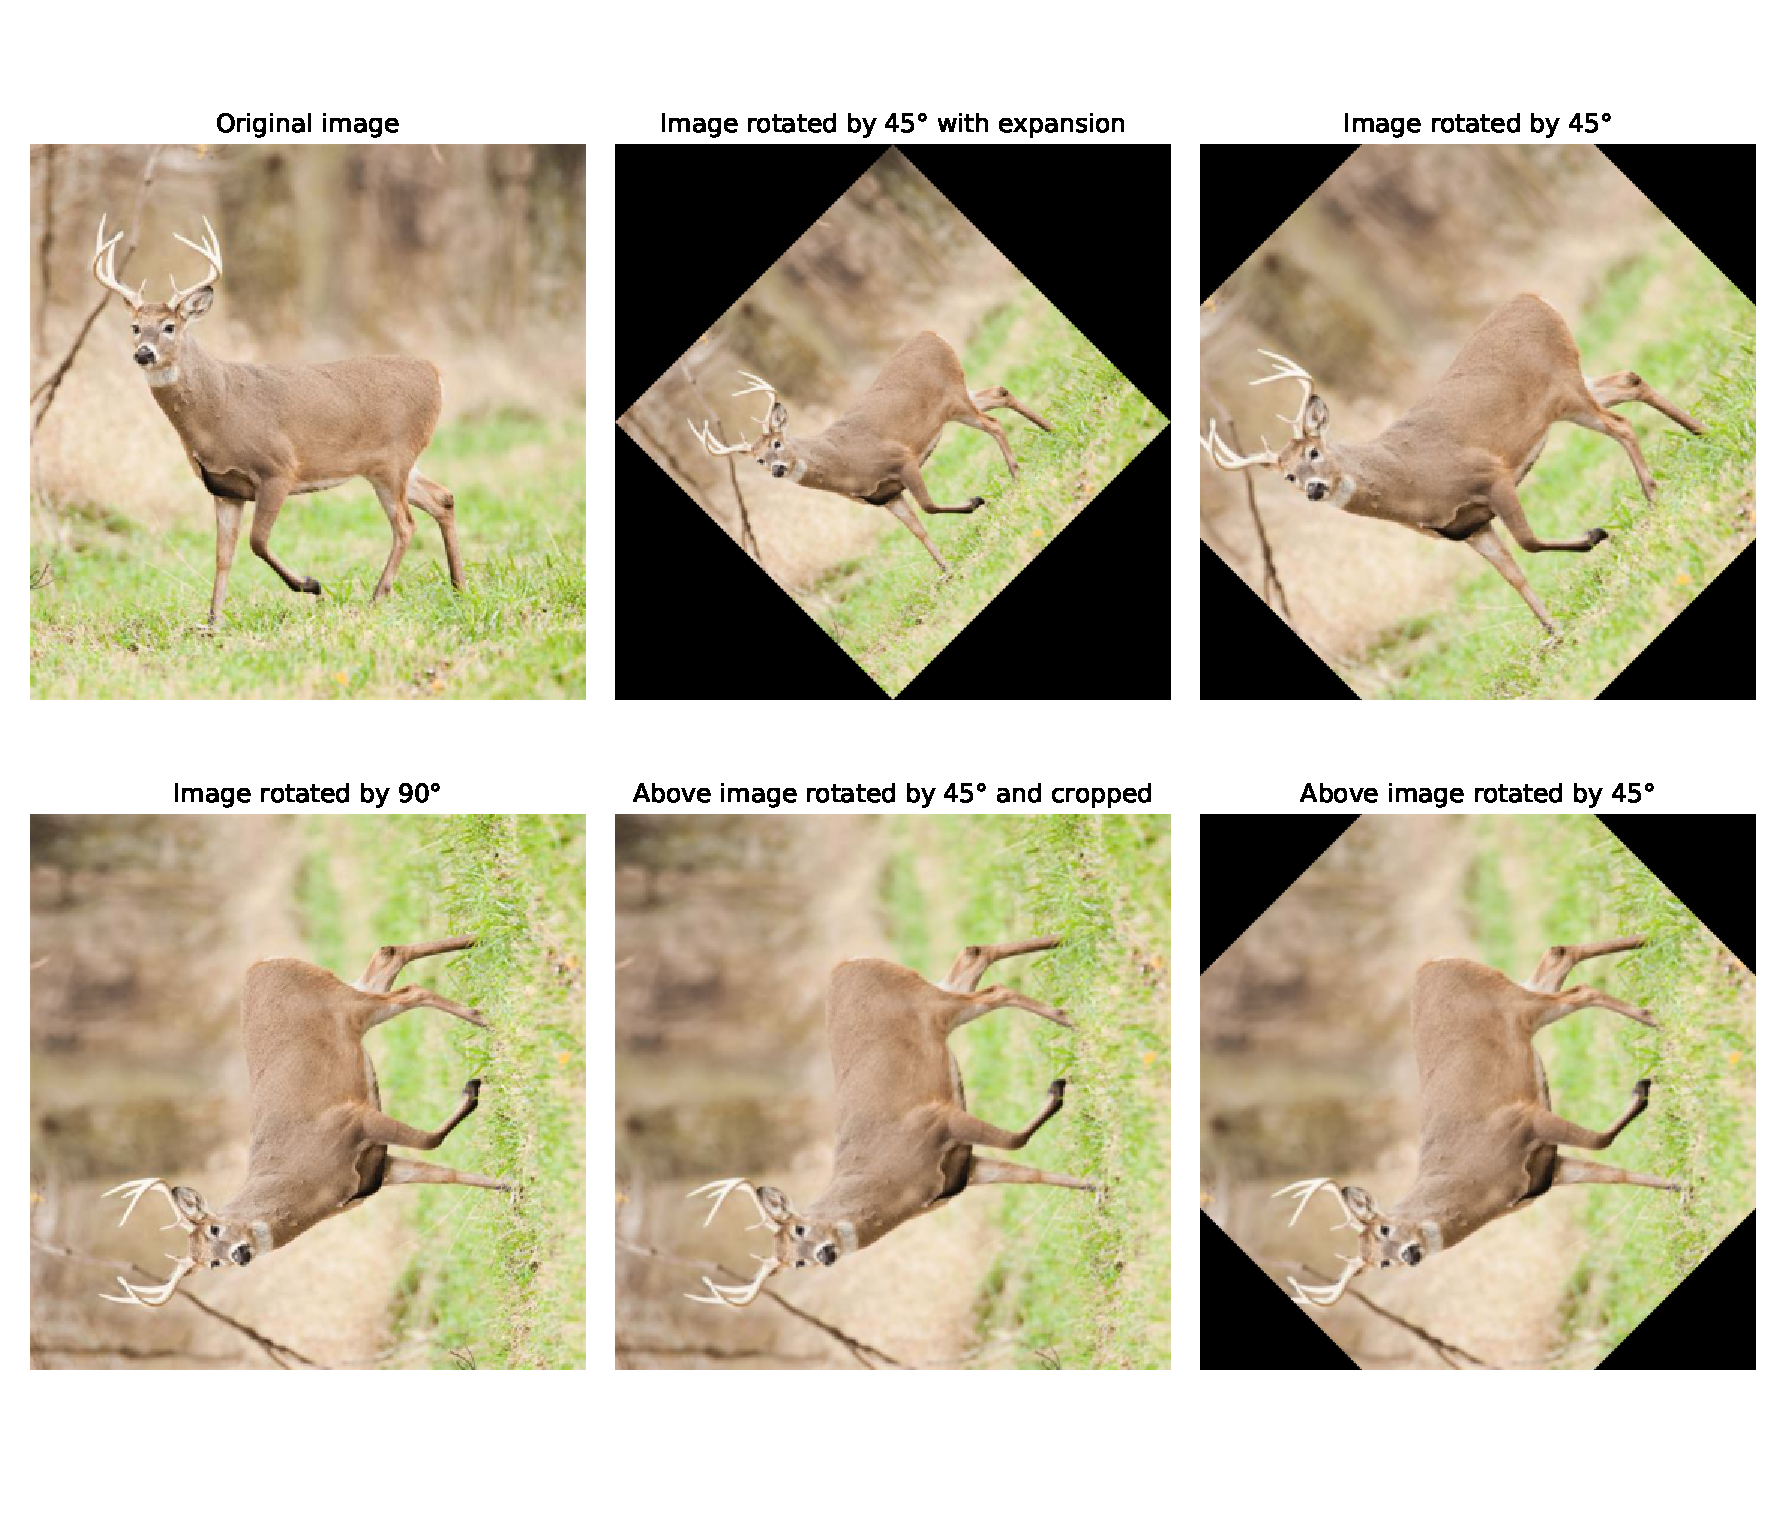
\includegraphics[width=\textwidth]{rotations}
            \caption{Difference between rotation with and without border
                expansion. Left column shows the original image and it's
                rotation by 90\degree. In middle column image is first rotated
                by 45\degree with expansion, then rotated again and cropped to
                original size. In the right column picture is simply rotated
                twice by 45\degree.}
            \label{fig:rotation_pics}
        \end{figure}
        While filters present in GCNNs are higher dimensional than in regular
        CNNs, spatial interpretation of the last two dimensions remains
        unchanged. Therefore it makes sense to generalize $\mathcal{R}$ to
        transform N-dimensional tensor by separately rotating last two
        dimensions of every subtensor and stacking them in original shape.
        The same goes for scaling and shear transformations described next.

    \subsubsection{Scaling}
        Scaling is a zoom-in or zoom-out transformation in reference to the
        center of the image. Scaling of coordinates can be written as
        \begin{equation}
            \mathcal{S}_k = \begin{bmatrix}
                k & 0 \\
                0 & k
            \end{bmatrix}
        \end{equation}
        Just like in rotation, after rescaling of coordinates, image needs to be
        resampled.
        Figure \ref{fig:scalings} shows varying degree of scaling.
        Note that by default scaling-up causes loss of
        information, so we might want to use image expansion as well.
        However while using finite expansion (increasing image size by at most
        $\sqrt{2}$) we can make rotations into a group action,
        it's not the case for scaling. In order to preserve all information
        during scaling by factor of $k>1$, we would have to increase image
        size by the same factor. For this reason scaling is often modeled not as
        a group, but rather as a semi-group or monoid. However it's not really any
        obstacle -- what matters is that locally it still has structure of a Lie
        group.


        \newcommand{\scalepic}[2]{
            \begin{subfigure}{#2\textwidth}
                \includegraphics[width=\linewidth]{{scalings/#1}.jpg}
            \end{subfigure}}
        \newcommand{\scalepiccaption}[3]{
            \begin{subfigure}{#2\textwidth}
                \includegraphics[width=\linewidth]{{scalings/#1}.jpg}
                \caption*{$k=#3$}
            \end{subfigure}}

        \begin{figure}[h]
            \centering
            \foreach \n in {0.5,0.75,1,1.5,2}
                {\scalepic{0temp\n}{0.18}} \\
            \foreach \n in {0.5,0.75,1,1.5,2}
                {\scalepic{121temp\n}{0.18}} \\
            \foreach \n in {0.5,0.75,1,1.5,2}
                {\scalepiccaption{105temp\n}{0.18}{\n}}

            \caption{Images from STL10 dataset with scaled by a factor of $k$.}
            \label{fig:scalings}
        \end{figure}

    \subsubsection{Shear}
        Shear operator `tilts' the coordinates. If we use the standard coordinate
        system centered  in the middle of the image,
        the first vector $e_1$ remains unchanged while $e_2$ is mapped
        to $\lambda e_1 + e_2$:
        \begin{equation}
        \mathcal{SH}_\lambda = \begin{bmatrix}
                1 & \lambda \\
                0 & 1
            \end{bmatrix}
        \end{equation}
        where $\lambda \in \mathbb{R}$. Parameter $\lambda$ is theoretically
        unbounded so the remarks from scaling section apply here as well. In
        practice however $\lambda = \pm -1$ causes tilt of $45 \degree$ which is
        already very significant so we only consider $\lambda \in [-1;1]$.
        Exemplary effect of transformation is shown in figure \ref{fig:shears}.

        \newcommand{\shearpic}[2]{
            \begin{subfigure}{#2\textwidth}
                \includegraphics[width=\linewidth]{{shears/#1}.jpg}
            \end{subfigure}}
        \newcommand{\shearpiccaption}[3]{
            \begin{subfigure}{#2\textwidth}
                \includegraphics[width=\linewidth]{{shears/#1}.jpg}
                \caption*{$\lambda=#3$}
            \end{subfigure}}

        \begin{figure}[h]
            \centering
            \foreach \n in {-1,-0.5,0,0.5,1}
                {\shearpic{0temp\n}{0.18}} \\
            \foreach \n in {-1,-0.5,0,0.5,1}
                {\shearpic{121temp\n}{0.18}} \\
            \foreach \n in {-1,-0.5,0,0.5,1}
                {\shearpiccaption{105temp\n}{0.18}{\n}}

                \caption{Images from STL10 dataset transformed by
                $\mathcal{SH}_\lambda$ for varying $\lambda$.}
            \label{fig:shears}
        \end{figure}


\section{Image symmetry implementation}
\newcommand\cbw{\mathit{CBW}}
\newcommand\gbw{\mathit{GBW}}

\subsection{Invariant Layers}
\subsubsection{CBW Layer}
As described in \ref{sec:theoretical_equiinv}, in order to construct a network
invariant to some group of transformations, either the first layer has to be
invariant or first layers have to be equivariant with an invariant layer
following them. In this section we construct networks of both of these types.
First we need to construct layers invariant to changes in
contrast, brightness, color balance and gamma correction as defined in
\ref{sec:transformations}. If possible it would be best to use a single function
invariant to all of these transformations at once. Fortunately such layer
exists. We show that simple instance normalization has this property.
Instance normalization layer $\mathit{CBW}$ transforms each channel
$X_c$ of image $X$ by:
$$ \mathit{CBW}(X_c) = \frac{X_c-E[X_c]}{\sigma(X_c)} $$
where $E[X_c]$ is mean value of $X_c$.
Each instance in batch is normalized separately.
\textit{CBW} is invariant to changes in contrast $\mcc$:
\begin{align*}
    \mathit{CBW}(\mcc_a(X)_c) &=
    \frac{aX_c+(1-a)E[X]_c - E\left[aX_c+(1-a)E[X]_c\right]}{\sigma(aX_c+(1-a)E[X]_c)} \\
    &= \frac{aX_c+(1-a)E[X]_c - aE[X_c]-(1-a)E[X]_c}{a\sigma(X_c)} \\
    &= \frac{aX_c-aE[X_c]}{a\sigma(X_c)} \\
    &= \frac{X_c-E[X_c]}{\sigma(X_c)} \\
    &= \mathit{CBW}(X_c)
\end{align*}
Similarly for brightness changes $\mathcal{B}$:
\begin{align*}
    \mathit{CBW}(\mathcal{B}_a(X)_c) &=
    \frac{aX_c - E\left[aX\right]_c}{\sigma(aX_c)} \\
    &= \frac{aX-aE[X_c]}{a\sigma(X_c)} \\
    &= \frac{X_c-E[X_c]}{\sigma(X_c)} \\
    &= \mathit{CBW}(X_c)
\end{align*}
Whereas color balance changes $\mathcal{W}$ act on individual channels by simple
scaling so:
\begin{align*}
    \mathit{CBW}(\mathcal{W}_T(X)_c) &=
    \frac{T_cX_c - E\left[T_cX_c\right]}{\sigma(T_cX_c)} = \\
    &= \frac{T_cX-T_cE[X_c]}{T_c\sigma(X_c)} = \\
    &= \frac{X_c-E[X_c]}{\sigma(X_c)} = \\
    &= \mathit{CBW}(X_c)
\end{align*}
Therefore any neural network with $\mathit{CBW}$ as first layer
makes the network invariant to considered image transformations.
We denote this type of networks as \{model-name\}+InCBW0, e.g. Plain+InCBW0 or
RotEq+InCBW0. Where 0 refers to placement of the invariant layer at the
beginning of the network. We also consider invariant networks with $\mathit{CBW}$
layer placed further down the processing stream. As mentioned earlier,
constructing such network requires all layers before $\mathit{CBW}$ to be
equivariant. Since the equivariance to changes in color balance is not defined,
we focus on contrast and brightness. In the next section \ref{sec:equ_models} we
present variants of common layers like convolution or pooling equivariant to
these transformations. We use these components to construct invariant networks
denoted InB1, InB2, InB3. Numbers again refer to
placement of the $\mathit{CBW}$ layer -- in InBn the invariant layer is placed
after Resnet's nth BasicBlock.

\subsubsection{GBW Layer}
Just like $\cbw$ layer is invariant to changes in contrast,
we can construct similar normalization layer $\gbw$ invariant to changes in
gamma:
\begin{equation}
    \gbw(X_c) = \frac{\log{X_c}-E[\log{X_c}]}{\sigma(\log{X_c})}
    \label{eq:GBW}
\end{equation}
where $\log(X)$ is entrywise logarithm of $X$. The base of the
logarithm is not very important -- invariant behaviour doesn't depend on it's value.
Now let us assume that we're given an image -- $3\times H \times W$ tensor --
with strictly positive values..
Operators $\mathcal{G}$, $\mathcal{B}$ and $\mathcal{W}$ act on it entrywise, so
we can as well analyze transformation of individual channels of the image.
Let $X$ be a single channel.
We prove \ref{eq:GBW} is invariant to gamma, brightness and color balance
changes. $\mathcal{B}$ and $\mathcal{W}$ transform single channel in the same
way, by multiplication,
so we only need proofs for $\mathcal{G}$ and $\mathcal{B}$:

\begin{align*}
    \gbw(\mathcal{G}_a(X)) &=
    \gbw(X^a) \\
    &= \frac{\log(X^a)-E[\log(X^a)]}{\sigma(\log(X^a))} \\
    &= \frac{a\log(X)-E[a\log(X)]}{\sigma(a\log(X))} \\
    &= \frac{a\log(X)-aE[\log(X)]}{a\sigma(\log(X))} \\
    &= \frac{\log(X)-E[\log(X)]}{\sigma(\log(X))} \\
    &= \gbw(X)
\end{align*}

\begin{align*}
    \gbw(\mathcal{B}_a(X)) &=
    \gbw(aX) \\
    &= \frac{\log(aX)-E[\log(aX)]}{\sigma(\log(aX))} \\
    &= \frac{\log(X)+\log(a)-E[\log(X)+\log(a)]}{\sigma(\log(X)+\log(a))} \\
    &= \frac{\log(X)+\log(a)-E[\log(X)]-\log(a)}{\sigma(\log(X))} \\
    &= \frac{\log(X)-E[\log(X)]}{\sigma(\log(X))} \\
    &= \gbw(X)
\end{align*}

There is however slight technical issue with definition \ref{eq:GBW}.
Since images contain values from interval $[0;1]$,
taking their logarithm directly is impossible because of
cells containing $0$. This problem is solved easily by adding some small constant value
$\epsilon$ to every cell before computing logarithm. The exact definition
is then in fact the following:
\begin{equation}
\gbw_{\epsilon}(X_c) =
    \frac{\log(X_c+\epsilon)-E[\log(X_c+\epsilon)]}{\sigma(\log(X_c+\epsilon))}
\end{equation}
To be precise, this small correction breaks the invariance properties,
%TODO: exact value of error
but fortunately the difference between the two layers is no
greater than $0.5\%$ (see section TODO), so we
can treat $\gbw_{\epsilon}$ as if it was also truly invariant.



\subsection{Equivariant models}
\label{sec:equ_models}

\subsubsection{Brightness equivariance}
Recall that layer $f$ is equivaraint to
change of brightness if $ f(aX) = af(X)$ for ant $a>0$.
We begin with showing that common building blocks of CNNs except for
normalization fulfill this condition:
\begin{itemize}
    \item \textbf{Convolution} is linear operation so $\mathit{Conv}(aX) =
        a\mathit{Conv}(X)$
    \item \textbf{Pooling} - all commonly used pooling layers are equivariant:
        \begin{itemize}
            \item MaxPooling amounts to taking maximal value of some set and\\
                $\max\{ax_1,ax_2,\cdots,ax_n\}=a\max\{x_1,x_2,\cdots,x_n\}$
            \item AveragePooling is precisely expectation operation $E[X]$ and
                    $E[aX] = aE[X]$
            \item EuclideanNormPooling -
                $\sqrt{(ax_1)^2+\cdots+(ax_n)^2} = a\sqrt{x_1^2+\cdots+x_n^2}$
        \end{itemize}
    \item \textbf{Activation functions} -- equivariant pointwise activation
        function is characterised by equation $f(ax) = af(x)$ for all $a>0$.
        Assuming $f$ is differentiable, $af'(ax) = af'(x)$, so $f'(ax)=f'(x)$ which
        means that $f'(a)=f'(1)$ for $a>0$ and $f'(b)=f'(-1)$ for $b<0$.
        This implies $f$ has form of generalized ReLU function
        $$f(x)=\left\{
            \begin{array}{lll}
                ax & \mbox{for some } a \in \mathbb{R} & \mbox{if } x<0 \\
                bx & \mbox{for some } b \in \mathbb{R} & \mbox{if } x \geq 0
            \end{array}\right.$$
        In particular we can use usual ReLU function.
    \item \textbf{Normalization} As shown above, instance normalization is
        invariant to brightness changes. It's easy to see that it also holds
        for Batch Normalization. This stems mainly from division by
        standard deviation which is equivariant to $\mathcal{B}$. In fact
        the numerator of $\mathit{CBW}$ is also equivariant to $\mathcal{B}_a$:
        $aX_c-E[aX_c]=a(X_c-E[X_c])$, so division by any factor involving $a$
        will break equivariance. For the same reason, we can't use pass the
        numerator through any nonlinear function, e.g. square root.
        Therefore if we want the normalization to zero
        out mean value of input, we must divide by a constant. This might have
        adverse effect on network's training since there is no mechanism to keep
        values flowing through the network bounded, which might easily result in
        gradient explosion. We compare norms of gradients in {\color{red}TODO}.
\end{itemize}
And so using common components with standard normalization scheme replaced by
mean normalization we can build model equivariant to brightness changes. In
experiments refer to this type of architecture as Brightness-Eq.

\subsubsection{Geometric transformations equivariance}
\label{sec:geom_eq}

\subsubsection{Gamma and contrast equivariance}
As expected from definitions, operators $\mathcal{C}$ and $\mathcal{G}$ are not
as well-behaved as $\mathcal{B}$. While MaxPooling remains equivariant, the rest
of described above layers doesn't (see experiments in section TODO).
For the rest of this section we construct suitable
convolutional layers similar to those of Lie
GCNNs (section \ref{sec:lie_gcnn}),
activation fucntions and
normalization layers
equivaraint to $\mathcal{C}$ and $\mathcal{G}$.

\begin{itemize}
\item
The crucial part of pipeline is convolution layer. Note that nature of geometric
and lighnig symmetries is fundamentally mathematically different. While the
transforms coordinates or grid of image, the latter group acts posintwise on
values present in the tensor without changing coordinates in any way.
This property renders the implementation used in \ref{sec:geom_eq} unfit.
Where in case of geometric symmetries different transformed locations
on original grid are sampled, in case of lightning symmetries these woulb be the
exact same locations. This in turn would cause creation of identical kernels and
unncesery repetition of computation. Therefore it's obligatory to transoform the
kernels in some other way consistent with abstract equations of lifting and convolution.
We implement it using the transformations from transformation group.
That is if we want the layer to be equivariant with respect to
$\mathcal{G}_c$, then it's kernel $K$ assumes values at gamma level $c$ equal to
base kernel gamma-corrected by factor of $c$:
\begin{equation}
    K(g) = K(x,c) = \mathcal{G}_c(K(x,0))
\end{equation}

\item Because of aggregation of gloabl mean of tensor in \ref{eq:contrast},
    designing a nontrivial pointwise activation function equivaraint to \ref{eq:contrast}
    might be impossible -- value in any given cell would automatically depend on
    values of all other cells. Instead we test numerically equivariance of broad
    range of popular activation functions and find that function Softsign
    defined as $\mathit{Softsign}(x) = \frac{x}{1+|x|}$ performs fairly well.
    Exact measurements can be found in section TODO.

    Operator $\mathcal{G}$ proves to be more managable and exactly equivaraint
    activation function can be found, though in the end it turns out to be
    fairly obvious. If we want $f$ to be equivaraint to \ref{eq:gamma}, then in
    particular it needs to fulfill condition $$f\left(x^c\right) =
    f\left(x\right)^c$$
    for any $x>0$ and
    $c > 0$. To obtain analytic form of $f$
    let $$f(x_0)=y_0$$ for some constants $x_0 \neq 1$ and $y_0$.
    Then $$f\left(x_0^c\right) = y_0^c$$ Now we can treat $x_0^c$ as the argument and set
    $x_0^c = z$, so $$f(z) = y_0^{\log_{x_0}z}$$.
\end{itemize}







\section{Experiments}
\subsection{Experimental setup}
    \subsubsection{Used technologies}
    \subsubsection{Datasets}
    \subsubsection{Models}

\subsection{Image classification}

\subsection{Degree of equivariance and invariance}



% -- bibliography --
\printbibliography

%% -- list of figures and tables --
\clearpage
\listoffigures
\listoftables

\end{document}

